
\chapter{Causal units}
\label{causalunits}
%\begin{quotation}
%Everything is this way because it got this way. 
%\textit{D'Arcy Thompson}
%\end{quotation}



What is the causal relationship between the bits of language --- sounds, words, idioms --- and the whole systems that we call languages? A way into this question is to ask why any two languages might share a trait. There are four possible reasons: %(Enfield 2003:368)


\begin{enumerate}
\item[0.] {\textit{Universal presence}: All languages must have the trait; therefore A and B have it.}

\item[1.] {\textit{Vertical transmission}\is{vertical transmission}: The trait was inherited into both A and B from a single common ancestor language.} 

\item[2.] {\textit{Horizontal transmission}\is{horizontal transmission}: The trait was borrowed into one or both of the languages (from A into B, from B into A, or from a third language into both A and B). }

\item[3.] {\textit{Internal development}\is{internal change}: The trait was internally innovated by both A and B, independent from each other.}\footnote{If the two languages possessed the same starting conditions for the same internal innovation, the question arises as to why they shared those starting conditions in the first place. This takes us back to the question \textquoteleft Why do two languages share a trait?'.}

\end{enumerate}

%Anyone who has grappled with the problem of language contact and its historical effects will know the conceptual problems that arise from this question. Consider some of the many examples from around the world of neighbouring but unrelated languages that show many traits in common:

%\begin{enumerate}
%\item 1.	In Northern California, native American languages of different stocks share features including phonetic/phonological systems and processes, MORE (REF);
%\item 2.	In Mesoamerica, languages of different stocks share features including head-marking possessive constructions, relational nouns, and vigesimal numeral systems (REF);
%\item 3.	In South Asia, languages of different stocks share features including retroflex consonants, conjunctive participles, (inter alia) among different stocks in .
%\item 4.	In the Balkans, languages of different stocks share features including post-posed articles, loss of infinitive in complement clauses, vowel harmony (inter alia).
%\item 5. 	In mainland Southeast Asia, languages of different stocks share features including (Enfield and Comrie 2015:7--8; cf. Enfield 2003, 2005);
%\end{enumerate}


%The phenomena of language contact is usually discussed in terms of the properties of languages --- what features languages have, how languages affect each other, what happens to languages. But if the empirical validity of the unit \textquoteleft language' as a causal entity is not a given, then we must wonder whether items are all we have.

Leaving aside universals, the three possibilities (1--3) involve processes that are often considered to be qualitatively different, namely (1) inheritance\is{inheritance} (from mother to daughter language), (2) borrowing\is{borrowing} (from neighbouring language to neighbouring language through contact\is{language contact} among speakers), and (3) natural, internally motivated development. But at a fundamental level these processes are not distinct: 


\begin{quotation}
Language change by contact or otherwise is a process of social diffusion. The standard analytical distinction between internal and external linguistic mechanisms diverts attention from the fact that these are instances of the same process: the diffusion of cultural innovation in human populations. \citep[197]{enfield_areal_2005}

\end{quotation}

This is the conclusion I came to when considering possible explanations for convergence of structure among neighboring language communities in the mainland Southeast Asia\is{mainland Southeast Asia} area. As I put it then:

%\begin{quotation}
%All language change, whether by genealogical inheritance or areal diffusion, is conducted by a process of social diffusion of innovation. Once this is acknowledged, the analytical distinction between inheritance and diffusion begins to crumble. %Nevertheless, the genealogical method remains a useful descriptive technique.
%\end{quotation}

\begin{quotation}
Areal linguistics\is{areal linguistics} invites us to revise our understanding of the ontology of languages and their historical evolution, showing that the only units one needs to posit as playing a causal role are individual speakers and individual linguistic items. These unit types are mobile or detachable with respect to the populations they inhabit, arguing against essentialism\is{essentialism} in both linguistic and sociocultural systems. 
\end{quotation}


\begin{quotation}
Areal linguistics presents significant challenges for standard understandings of the ontology of language\is{ontology of language} from both spatial and temporal perspectives. Scholars of language need to work through the implications of the view that \textquoteleft the language' and \textquoteleft the community' are incoherent as units of analysis for causal processes in the historical and areal trajectories of language diffusion and change.  \citep[198]{enfield_areal_2005}
\end{quotation}

%Earlier (Enfield 2003: 368), regarding the oft-made distinction between inheritance of the same trait from a common ancestor, borrowing of a trait across languages, and parallel but independent internal development as accounts for similarity between languages, I wrote: 


%\begin{quotation}
%At a fundamental level, these three channels of a sign's entry into a language [i.e., inheritance, borrowing, internal development] are indistinguishable.
%\end{quotation}


In this book I explore some implications of these conclusions. When we grapple with puzzles of inheritance, contact, and diffusion in the history of languages, we have to confront the item/system problem\is{item/system problem} (see Chapter \ref{itemsystemproblem}), and its collateral challenges.  
%\footnote{Some approaches work with related ideas using computational methods such as agent-based modeling and bioinformatics, and applying the concepts of evolutionary biology (e.g., \citealt{kirby_cumulative_2008,dunn_aslian_2011}). The causal account proposed here is at the conceptual level, and is independent from the specific methods used. While the application of bioinformatic methods is beyond the scope of this work, the framework and findings would ideally lead to close exchange with those approaches.}
 
The three processes mentioned above --- inheritance\is{inheritance}, borrowing\is{borrowing}, innovation\is{innovation} --- can only take place when there is social contact between people, and successful diffusion of types of behaviour in communities. These are causal preconditions. For any of the three processes to succeed, several things have to happen. People have to start saying things in new ways (or saying new things), exposing others in their personal network to new ideas. Those who are exposed then have to copy this new behavior, and they have to be motivated to do so. This in turn has to expose more people in their social networks, as well as further exposing those who began the process in the first place, validating and encouraging the new behaviour, and leading it to take further hold. At a fundamental level, the three ways that something can get into a language are indistinguishable from one another. If there are differences, they have to do with where the idea came from, how natural the idea is (i.e. how much it makes sense and perhaps how much it helps cut corners in communication\is{communication} or processing\is{processing}), and what is the social identificational value of the idea.


\section{How we represent language change}

One way to understand something is to look at the history of events that created it. Consider the history of any type of life form\is{life forms}. The central formative events take place in populations. Individuals inherit characteristics --- for example, from the genome\is{genetics} of their parents --- and when those inherited characteristics can vary between individuals in a population, an individual with one variant might have a better chance of surviving than someone with another variant. When higher likelihood of survival means higher likelihood of reproduction\is{reproduction}, this can increase the frequency of an advantageous variant in the population. In time, the variant comes to be carried by all individuals. Two or more distinct populations emerge, and these may then be regarded as separate species\is{speciation}. While the new populations share a common ancestor, they are now essentially different.

This way of thinking about the causal basis of species in terms of population dynamics is central in the theory of biological evolution \citep{darwin_origin_1859,mayr_populations_1970}. It can be applied to the evolution\is{evolution!biological} of life forms of all kinds, and to cultural types including kinship systems, technologies, and languages \citep{dawkins_selfish_1976,mesoudi_towards_2006}. The process of speciation in any of these forms of life implies relations of common ancestry that may be represented using a tree diagram\is{tree diagrams}. Figure \ref{treediagram} illustrates.

\begin{figure}[h]
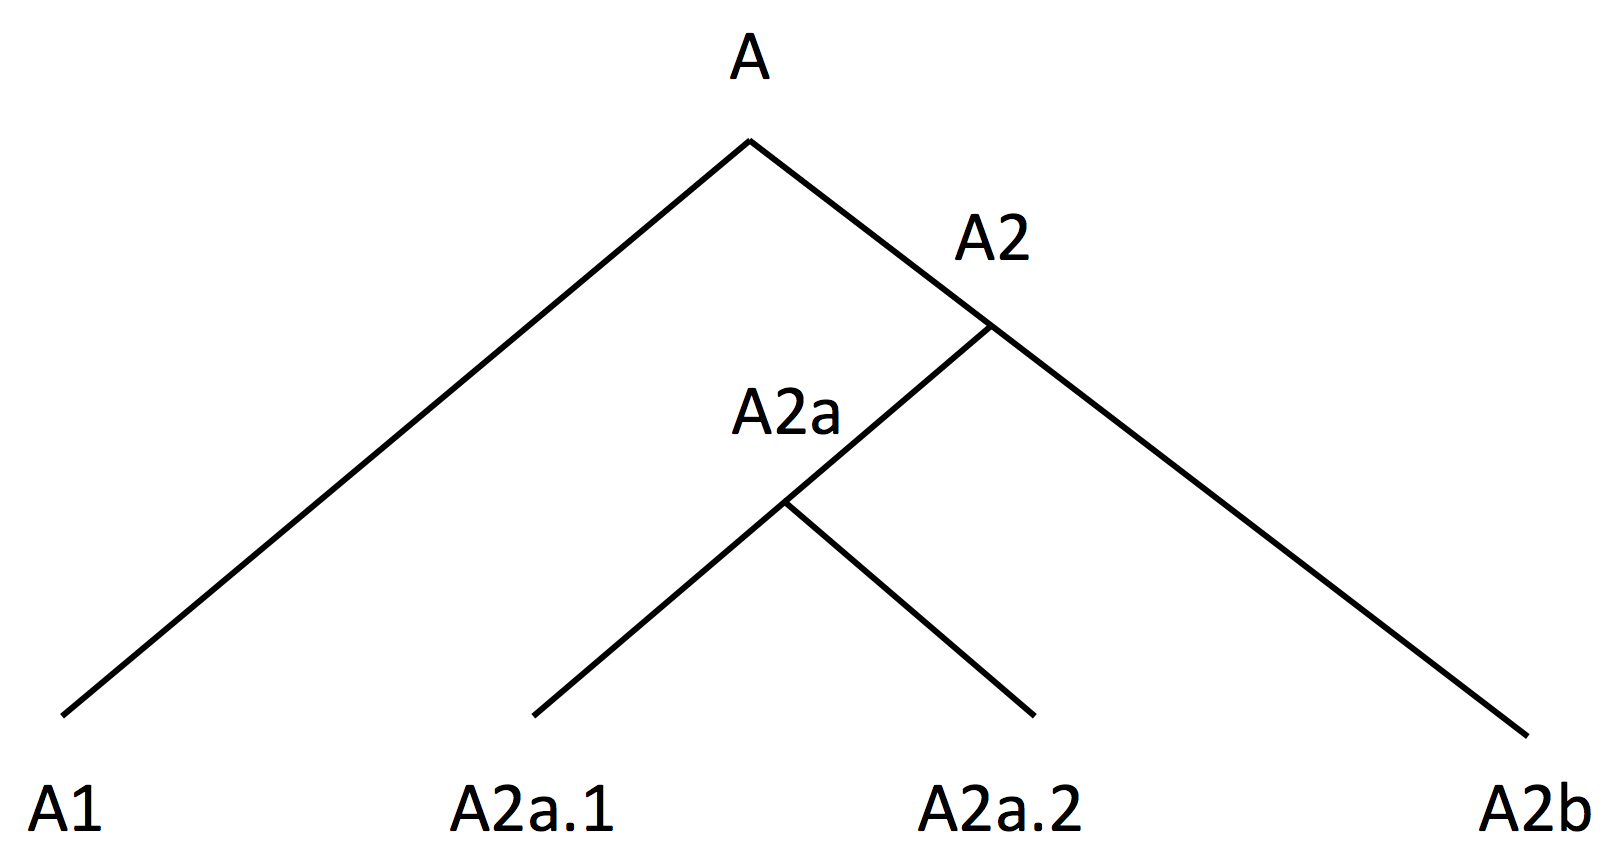
\includegraphics[width=0.60\textwidth,keepaspectratio]{figures/FigTree}
\caption{Tree diagram representing divergence by descent with modification. A1, A2a.1, A2a.2, and A2b are common descendants of A.}
\label{treediagram}
\end{figure}

Diversification of languages, as in the history of great stocks like Bantu\is{Bantu language family}, Austronesian\is{Austronesian language family}, and Indo-European,\is{Indo-European language family} has long been represented with tree diagrams of this kind, in which the ostensible units of analysis are languages. By taking the language as the unit of analysis, tree diagrams must assume that languages cohere as units. Is this a fair assumption? Are language systems coherent, natural kinds? Or do we only imagine them to be? 

 

%Language history does show some causal biases toward vertical transmission, and our research needs to determine and account for the nature of these biases (see Chapter 4, below). But biases toward vertical transmission are significantly weaker than comparable biases in vertebrate lineages in biology. Historical processes in language differ in two fundamental ways from the kind of vertical transmission we see in the evolution of species in vertebrates. First, in addition to the vertical transmission that accounts for what is shared among daughter and parent languages, there is often extensive horizontal transmission, by which traits of a daughter language are neither inherited from a parent language nor internally innovated, but are adopted from a contact language. Nothing like this kind of horizontal transmission --- at least not on anything remotely like this scale --- occurs in the biological evolution of vertebrates. 

When tree diagrams are used to represent the history of diversification within a family of languages, there is an analogy with the kind of evolution\is{evolution!biological} seen in life forms that show a total or near-total bias toward vertical transmission in evolution, namely vertebrates\is{vertebrates} such as primates, birds, fish, and reptiles. So let us consider what the tree diagram means in the case of vertebrate natural history. Each binary branching in the tree represents a definitive split in a breeding population. The populations represented by daughter nodes inherit traits that were found in the parent population. Members of the daughter populations also commonly inherit modifications of the parent traits that significantly distinguish the two daughter populations from each other. Inheritance happens in events of sexual reproduction, in which complete genotypes are bestowed in the conception of new individuals. This encapsulation of the genome in causal events of inheritance ensures the vertical transmission that a tree diagram represents so well. In vertebrate species, when two populations are no longer able to interbreed, they can no longer contribute to each other's historical gene pool. This would be \textit{horizontal transmission},\is{horizontal transmission} something that is essentially absent from vertebrate evolution (though with some caveats; \citealt{koonin_darwinian_2009}). The tree representation is adequate in the case of vertebrate speciation\is{speciation} for one reason: the tree diagram does not capture horizontal transmission. The vertebrate genome\is{genetics} is essentially acquired by the individual organism as a bundle. So the complete organism can reasonably be treated as a unit for describing transmission and change in phylogeny\is{phylogenetic frame}. The vehicle for replication is the individual organism as defined by the structurally coherent entity that we call the body.

The problem is that while vertebrates have been implicitly taken to be the model for language, they are not like language in causal terms. They are not even representative of life forms\is{life forms} in general. Most forms of life, including not only the non-animal Eukaryotes, but also the Bacteria and Archaea, are not subject to strong vertical transmission\is{vertical transmission} constraints \citep{boto_horizontal_2010}. Most forms of life lack the bounded body plans that delineate vehicles or interactors for passing on replicable traits. The overall phenotypic structures of \textquoteleft individuals' in many species are to a large degree emergent. Evolutionary\is{evolution!biological} processes can be more clearly seen to operate on \textit{parts} of organisms \citep{dawkins_selfish_1976}.



\section{Linguistic systems}


People find it easy to accept \textquoteleft the language'\is{languages, as unit of analysis} as a unit of causal analysis. Our intuitions suggest that languages are effectively bounded, whole systems. We readily think of them as organisms. But they can also be thought of as focussed bundles of items. Indeed they should be thought of in this way, for the \textquoteleft linguistic system' is not a natural kind. 

The point has been made for linguistic systems with most clarity and rigor by \citet{le_page_acts_1985}. A prerequisite to the idea of a language (e.g. English) is the idea of a group of people who speak it. But as Le Page and Tabouret-Keller (\citeyear{le_page_acts_1985}) put it: 

\begin{quotation} Groups or communities and the linguistic attributes of such groups have no existential locus other than in the minds of individuals. (p. 4) We do not ourselves then need to put a boundary around any group of speakers and say \textquoteleft These are the speakers of Language A, different from Language B', except to the extent that the people think of themselves in that way, and identify with or distance themselves from others by their behaviour. (p. 9)
\end{quotation}

The point was made a half-century ago for social systems more generally by the anthropologist Edmund \citet{leach_political_1964}, in critiquing the structuralism of Radcliffe-Brown and students \citep{fortes_african_1940}: 

\begin{quotation}
Social systems were spoken of as if they were naturally existing real entities and the equilibrium inherent in such systems was intrinsic. (p. x)  I do not consider that social systems are a natural reality. In my view, the facts of ethnography and of history  can only \textit{appear} to be ordered in a systematic way if we impose upon these facts a figment of thought. (p. xii) 
\end{quotation}

Fair enough. But there must be some natural reality upon which we may impose our figments of thought. One candidate is the economy of \textit{bits} of language or culture, each of which has mobility: the words and other things that we can borrow from outside, without having to borrow the whole systems they come from. As \citet[22]{hudson_sociolinguistics_1996} puts it:

\begin{quotation}
We need to distance ourselves somewhat from the concepts represented by the words \textit{language} and \textit{dialect}, which are a reasonable reflection of our lay culture, called \textquoteleft common-sense knowledge', but not helpful in sociolinguistics. First, we need a term for the individual \textquoteleft bits of language' to which some sociolinguistic statements need to refer, where more global statements are not possible.
\end{quotation}

Hudson introduces \textit{linguistic item}\is{linguistic item} as a term for this unit with causal reality. Suppose that items --- in bundles --- are what we impose an essence upon when we imagine languages. Our vernacular language names would be labels for these imposed, imagined essences.\footnote{If the reader is concerned that the true holistic system nature of languages is being underestimated, see Chapter \ref{itemsystemproblem}, below.}


\section{Linguistic items}

The idea that languages are causally real units\is{languages, as unit of analysis} gets weaker when we think of the mechanisms of language transmission, both across and within generations. There are two problems for the language-as-real-system idea. The first is that causal processes of transmission can be observed most concretely operating upon items\is{linguistic items} (e.g., in the borrowing and learning of words), not on whole systems. The second is that horizontal transmission\is{horizontal transmission} occurs. All parts of a language appear in principle to be independently mobile (though of course some bits of language travel more freely than others; \citealt{thomason_language_1988,curnow_what_2001,thomason_language_2001}). Now consider these points more closely.

What is transmitted in language history? It is not the whole system at once, but the components of the system, piece by piece and chunk by chunk, in millions of distinct events. Never all at once but at separate moments, over days, weeks, months and years. To be sure, the result of language transmission is a high degree of overlap among idiolects\is{idiolects} in a human population.\footnote{On idiolect overlap or convergence, cf. \citet{bakhtin_dialogic_1981}, \citet[106--107, 157--158]{hockett_refurbishing_1987}, \citet[227--228]{lee_whorf_1996}.} The overlap is so high that our idiolects are practically indistinguishable. And this reassures us that systems are real wholes. How does this degree of idiolect overlap come about? 

Part of the answer is that speech communities\is{speech community} are inward-focused. People in a group transmit linguistic items when they converse and interact. This creates an economy of signs, in the sense of \citet{zipf_human_1949}. When people in a group interact repeatedly, more signs come to be shared among those people. And the more that signs are shared, the more readily those people interact. This feedback effect in the social circulation of linguistic items is both a result of, and a cause of, common ground\is{common ground} in a community. People have more common ground because they interact more; they interact more because they have more common ground. The basic causal units, though, are the shared items, not the systems that emerge.

The second problem with `the language' as a natural unit is the ease of borrowing\is{borrowing} linguistic items. Languages constantly incorporate new structures, and quickly. When confronted with this kind of horizontal transmission, students of language change have looked for ways to distinguish it from a vertical\is{vertical transmission} signal, usually to then exclude it. But if horizontal transmission\is{horizontal transmission} is so widespread, this should cause people to doubt the value of a model in which vertical transmission is the main object of interest for representing and understanding language history. With a proper understanding of the causality of language change, we see that tree diagrams\is{tree diagrams} that take \textquoteleft the language' as the unit of analysis not only abstract from reality, they distort it. They are poor conceptual tools for understanding the ontology of language.\is{ontology of language} The solution is to change our assumptions about the causal units involved.

For Darwinian\is{Darwin} evolution\is{evolution} to occur, there must be a population of essentially equivalent but non-identical units. These units must inherit traits from comparable units that existed prior to them. And these inheritable traits must show variation that can result in comparable units having different chances of surviving to pass on those traits to a new generation. What are the units? In the case of vertebrates, a received view is that two sorts of units work together: organisms, and genes. Organisms are vehicles for replicating genes\is{genetics}. In vertebrates\is{vertebrates}, the vehicles for inheritance of traits are the bodies of individuals. Each body is a phenotypic instantiation of the system. But here is the problem. The situation with languages is not like this at all. 


\section{Thinking causally about language change}
We want a causal account of languages as historically evolved systems. To think concretely about this, consider the following. All the conventional bits of language you learned as an infant\is{first language acquisition} were created by enormous chains of social interaction in the history of a population. Each link in the chain was an observable instance of usage, a micro-scale cycle of transmission, going from public (someone uses a structure when speaking) to private (a second person's mental state is affected when the structure is learnt or entrenched) and back to public (the second person uses the structure, exposing someone else), and so on. This may seem to be an overly micro-perspective way of putting it. But it is important to be explicit about the proximal mechanisms of transmission. Causal statements about language often highlight only a part of what is going on. 

Consider (1) and (2):


\begin{enumerate}
\item \textit{Knowledge of grammar causes instances of speaking.} 
\item \textit{Instances of speaking cause knowledge of grammar. }
\end{enumerate} 

Statement (1) focuses on competence\is{competence}. It points to mechanisms of, and prerequisites for, saying things. Statement (2) focuses on performance\is{performance} and emphasizes its outcomes. We learn about language from what people say. But there is no contradiction between the statements shown in (1) and (2). They are ways of framing the same thing. Competence and performance are equally indispensable in the processes of historical evolution that determine and constrain what a language can be like. Words are effectively competing for our selection\is{selection} \citep{croft_explaining_2000}. If all goes well, we select the items that best enable us to manipulate other people's attentional and interpretive resources \citep[16--17]{enfield_relationship_2013}. 

\section{The problem with tree diagrams}

Tree diagrams\is{tree diagrams} of language diversification are good for some things, but they are not good for representing causal processes of language history, nor the natural, causal ontology of languages and language relatedness.\is{ontology of language} The tree diagram assumes that we are primarily interested in one form of transmission of heritable characteristics, namely, vertical transmission\is{vertical transmission} of features from a parent to a daughter language, normally through first language acquisition\is{first language acquisition} in children. The alternative --- horizontal transmission\is{horizontal transmission}, i.e., transmission of features between languages whose speakers are in contact, normally involving adult language learning --- is acknowledged but is regarded as noise that needs to be factored out from the vertical historical signal of primary interest (cf. \citealt{dixon_rise_1997}, and note that some recent work applying new methods is showing promising signs of a shift in direction here; e.g., \citealt{reesink_explaining_2009}).

The tree diagram is a methodological simplification. It requires us to abstract from the causal facts. Of course this abstraction may be a harmless practical necessity. But our question is whether the abstraction inherent in the tree diagram does \textit{conceptual} harm. I think the answer is yes. It directs our attention away from the causal mechanisms that define language as an evolutionary process, and languages as evolved systems.

To begin to think causally we first need to explore the multiple frames within which causal processes may be effected. This is the topic of the next chapter. 

%\begin{list}{label}{spacing}
%\item (a) 	being exposed to semiotic material by which they may infer the idea; 

%(b) 	being motivated to infer the idea, and to actually create a representation of the idea; 

%(c) 	identifying as a person who would put the idea into practice;

%(d) 	putting the idea into practice, exposing others (back to (a)). 

%\end{list}





%If it is the material restrictions of time, space, social group size and the need for convention that create the very high levels of convergence in the linguistic behaviour and complex sign systems of social associates, then what accounts for the �system properties� of language, such as Greenbergian implicational universals? \textit{(The same question may be asked in anthropology generally, but linguistic anthropology allows us greater control.)} 


%Mead (1934:133) said �The processes of experience which the human brain makes possible are made possible only for a group of interacting individuals: only for individual organisms which are members of a society; not for the individual organism in isolation from other individual organisms�. (quoted in Rogoff 1990:14). See also Rosaldo (1984:145) for refs to Halliwell, Mead, Mauss and Fortes.

%Seeing that it is now widespread, we assume it has spread widely. This implies a time depth for the spreading process, as well as a source and direction of the spread. There is evidence of a process which may be described as epidemiology (Sperber 1985). People catch ideas for ways of saying things. Factors familiar to us from the field of sociolinguistics have licensed and constrained the transmission and adoption of new ways of saying things from one group of people to another. The current synchronic state is the outcome of such a process.

%The durability of signs is only maintained through constant field-testing of one's personal hypotheses about linguistic meaning. When you ask for \textit{salt} and get salt rather than pepper, your theory of the sign-category association <salt> is tested, confirmed, and therefore not revised. (There is no qualitative distinction, in this respect, between individual theories of the meanings of particular words, on the one hand, and grammatical categories, on the other.)


%\textit{The study of areal phenomena both force us to consider, and help us to answer, the central question of linguistics: What is the nature of language? What is the ontology of language?}



